\chapter{前言}
\renewcommand{\baselinestretch}{10.0} %設定行距
\pagenumbering{arabic} %設定頁號阿拉伯數字
\setcounter{page}{1}  %設定頁數
\fontsize{14pt}{2.5pt}\sectionef
\section{研究動機}
因為有越來越多的繪圖軟體加入,所以我們想試試用solid edge和femap畫出車門中控鎖內部零件,並做有限元素分析,來試試看它們對機械設計有何幫助\\

\begin{figure}[hbt!]
\begin{center}
\includegraphics[angle=90,width=10cm]{}
\caption{\Large }\label{fig.}
\end{center}
\end{figure}
\begin{figure}[hbt!]
\begin{center}
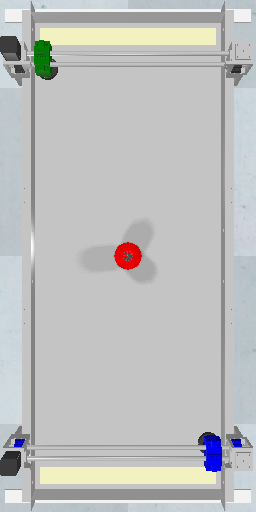
\includegraphics[angle=90,width=10cm]{origin}
\caption{\Large }\label{fig.}
\end{center}
\end{figure}
\begin{figure}[hbt!]
\begin{center}
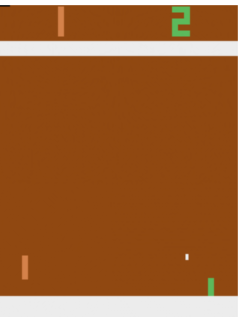
\includegraphics[height=8cm]{pong_gym}
\caption{\}\label{fig.}
\end{center}
\end{figure}


\section{研究目的與方法}
\\
 
 
\begin{figure}[hbt!]
\begin{center}
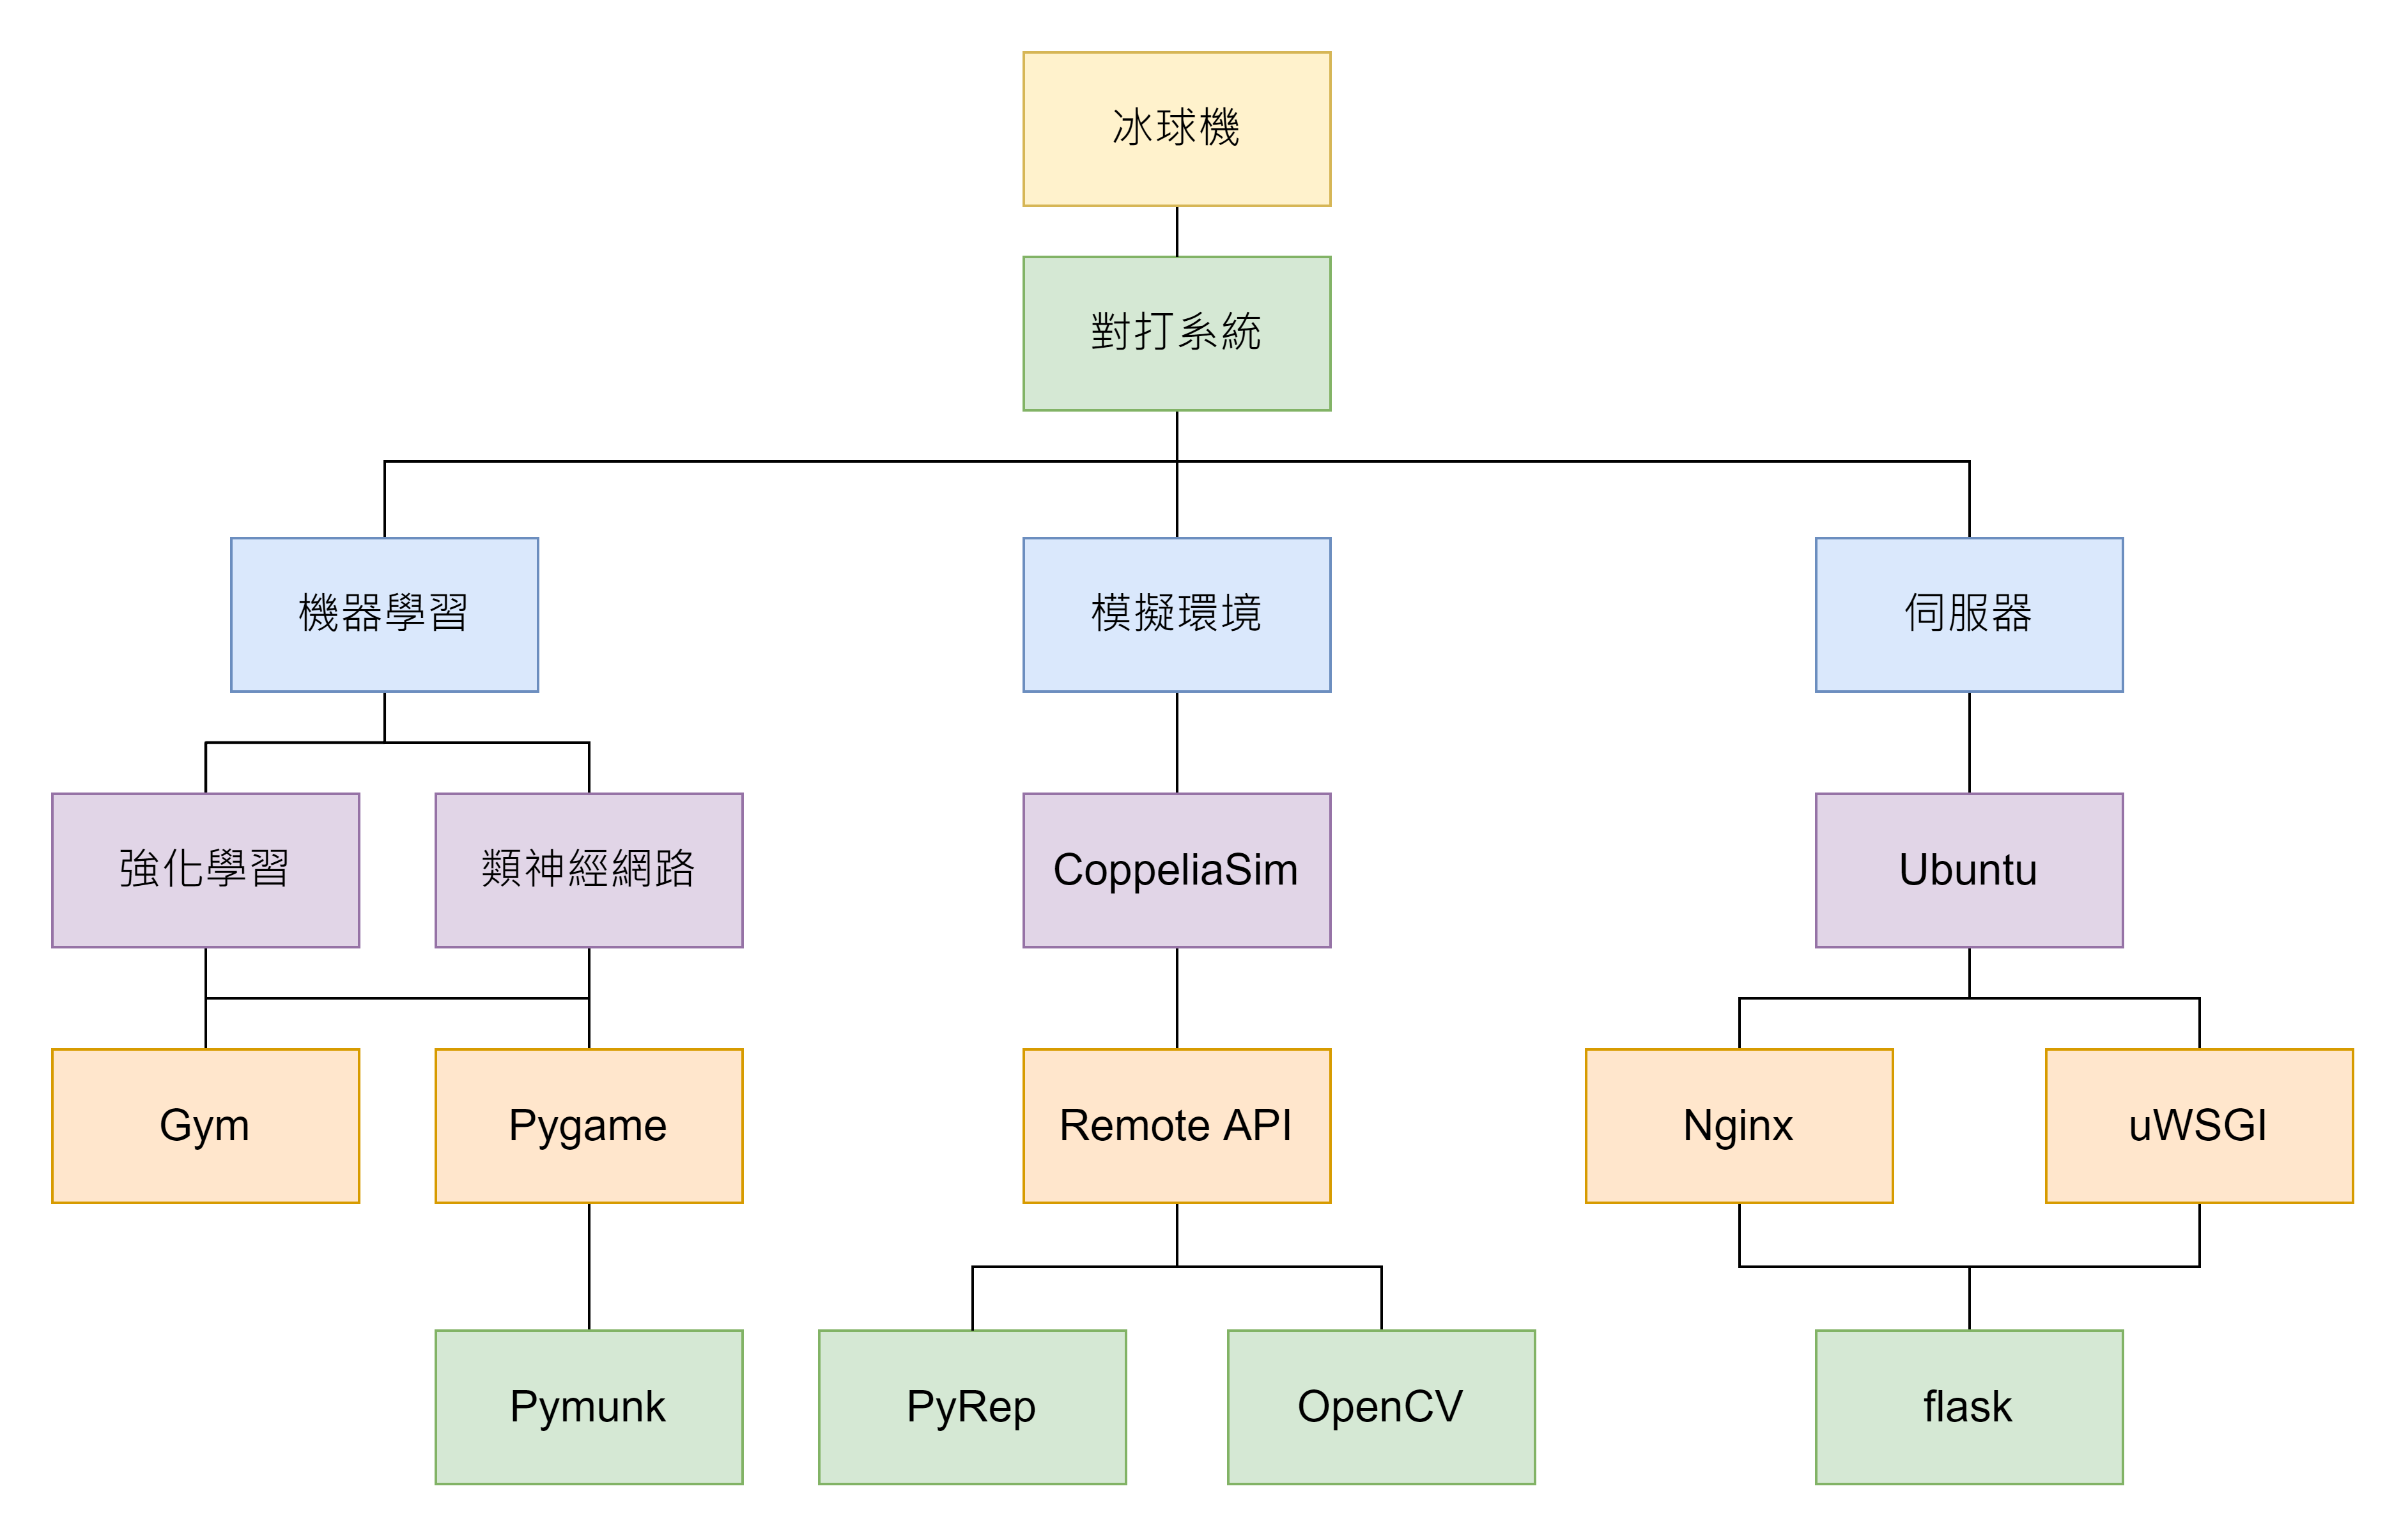
\includegraphics[width=15cm]{研究架構}
\caption{\Large 研究架構 }
\label{研究架構 }
\end{center}
\end{figure}
\section{未來展望}

\section{規則說明}
 
\begin{enumerate}
\item 
\item 
\item 
\end{enumerate}

\renewcommand{\baselinestretch}{0.5} %設定行距
